\documentclass{ntuabeamer}

\usepackage[utf8]{inputenc}
\usepackage{amsmath}
\usepackage{amssymb}
\usepackage{booktabs}
\usepackage{graphicx}
\usepackage{tikz}
\usepackage{appendixnumberbeamer}
\usepackage{pgfplots}
\pgfplotsset{compat=1.18}
\usetikzlibrary{arrows.meta,positioning}

\title{Generalization: Bias, Variance, and How to Control Them}
\author{}
\date{}
\graphicspath{{assets/}{assets/generated/}{assets/source/}}

\definecolor{courseblue}{HTML}{3F7CAC}
\definecolor{courseorange}{HTML}{D97706}
\definecolor{coursegreen}{HTML}{27864A}
\definecolor{coursepurple}{HTML}{7656A3}
\definecolor{coursered}{HTML}{B5473C}
\definecolor{coursegray}{HTML}{667085}
\definecolor{courselightblue}{HTML}{DCE9F5}
\definecolor{courselightorange}{HTML}{F9E4C8}

% One plain-sentence conclusion per frame.
\newcommand{\takeaway}[1]{\par\vspace{0.3cm}{\color{courseblue}\textbf{#1}}\par}

\begin{document}

\begin{frame}[plain]
  \makepresentationtitle
\end{frame}

% ------------------------------------------------------------------ fitting vs generalizing
\section{Underfitting and Overfitting}
\sectiondivider{Underfitting and Overfitting}

\begin{frame}{What We Really Want: Good Predictions on New Data}
  \[
    L_D(\theta)=\frac1n\sum_{i=1}^n\ell(f_\theta(x_i),y_i),
    \qquad R(\theta)=\mathbb E_{(X,Y)}\ell(f_\theta(X),Y).
  \]
  $L_D$ is measured on the examples used for fitting; $R$ is the loss on a new draw from the same source. A held-out set estimates $R$.
  \takeaway{Low training loss can coexist with high new-data loss when a flexible fit follows sample noise.}
\end{frame}

\begin{frame}{Underfit, Good Fit, Overfit}
  \centering
  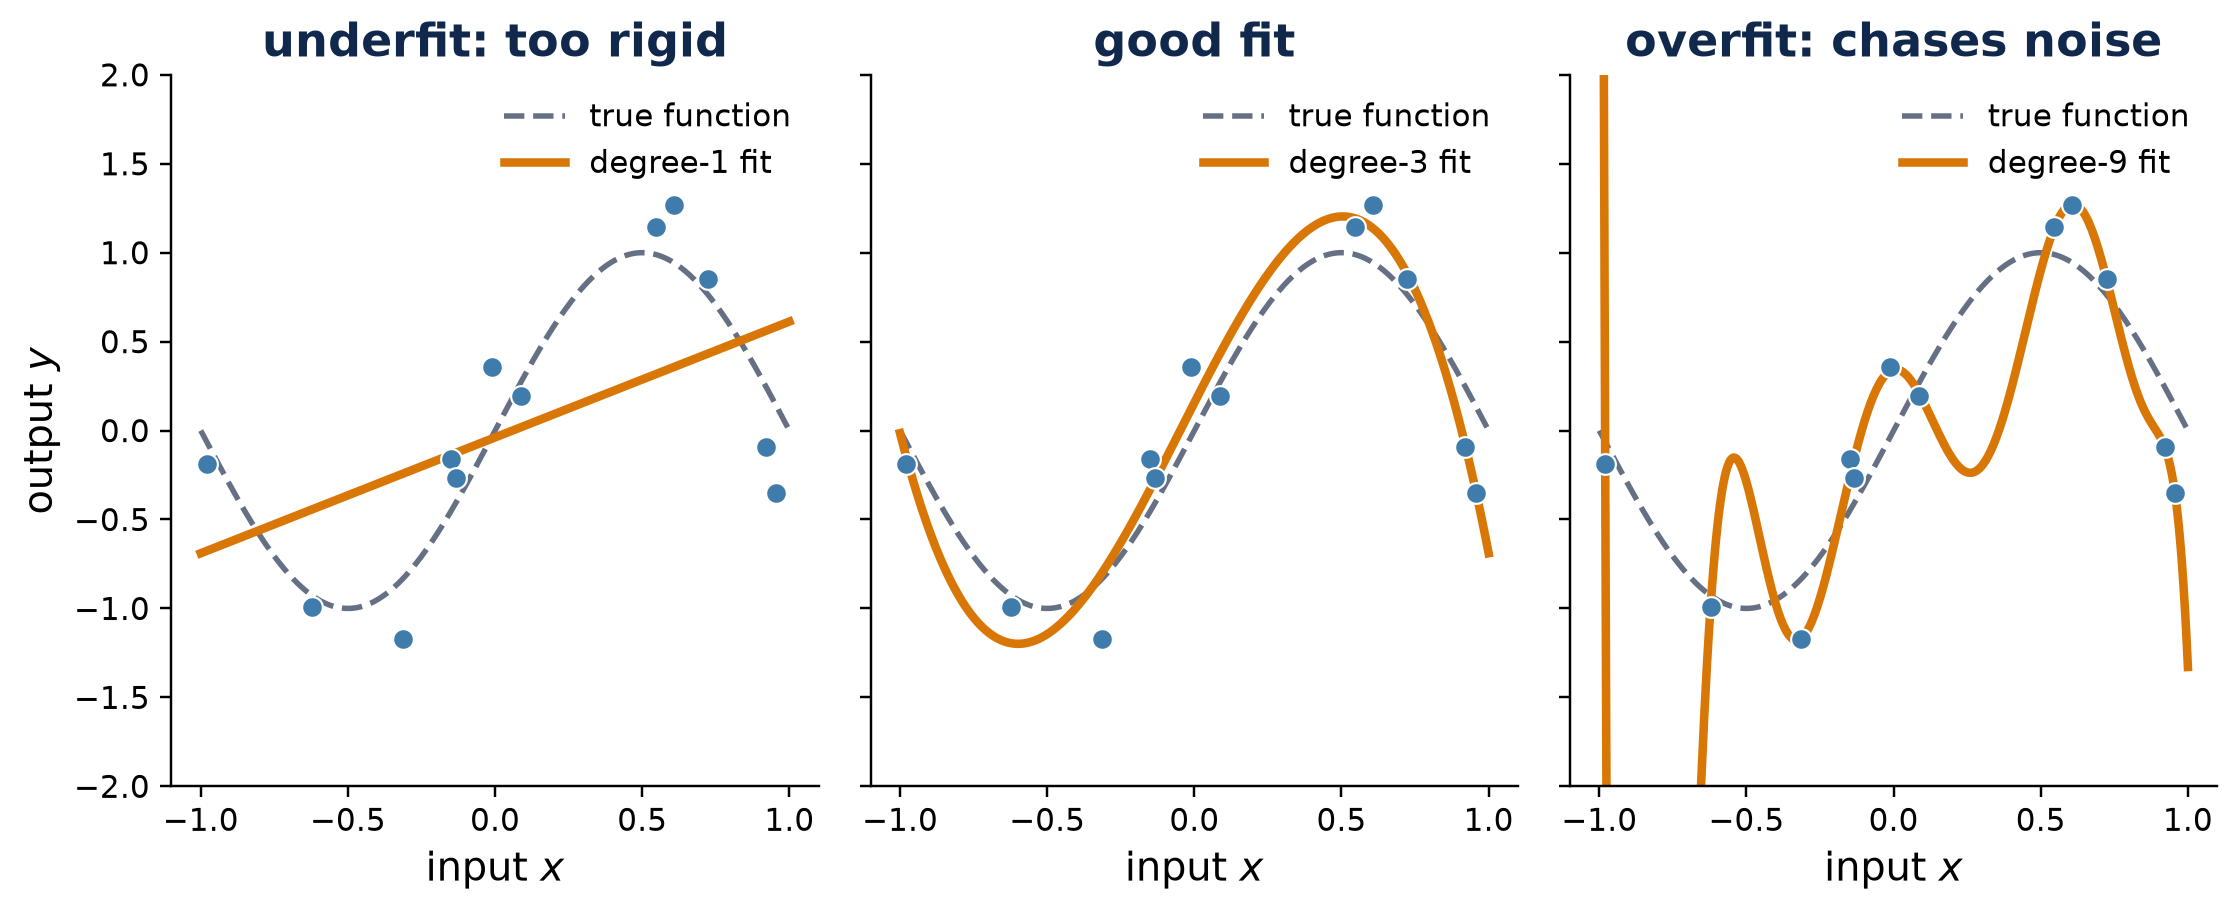
\includegraphics[width=0.98\linewidth,height=0.5\textheight,keepaspectratio]{fit-regimes.png}

  \small Same 12 noisy points, three models of increasing flexibility (a straight line, a cubic, a degree-9 polynomial).
  The degree-9 curve leaves the plot at the left edge.
  \takeaway{So: too rigid misses the pattern, too flexible chases the noise.}
\end{frame}

\begin{frame}{More Flexibility Always Helps Training, Not New Data}
  \centering
  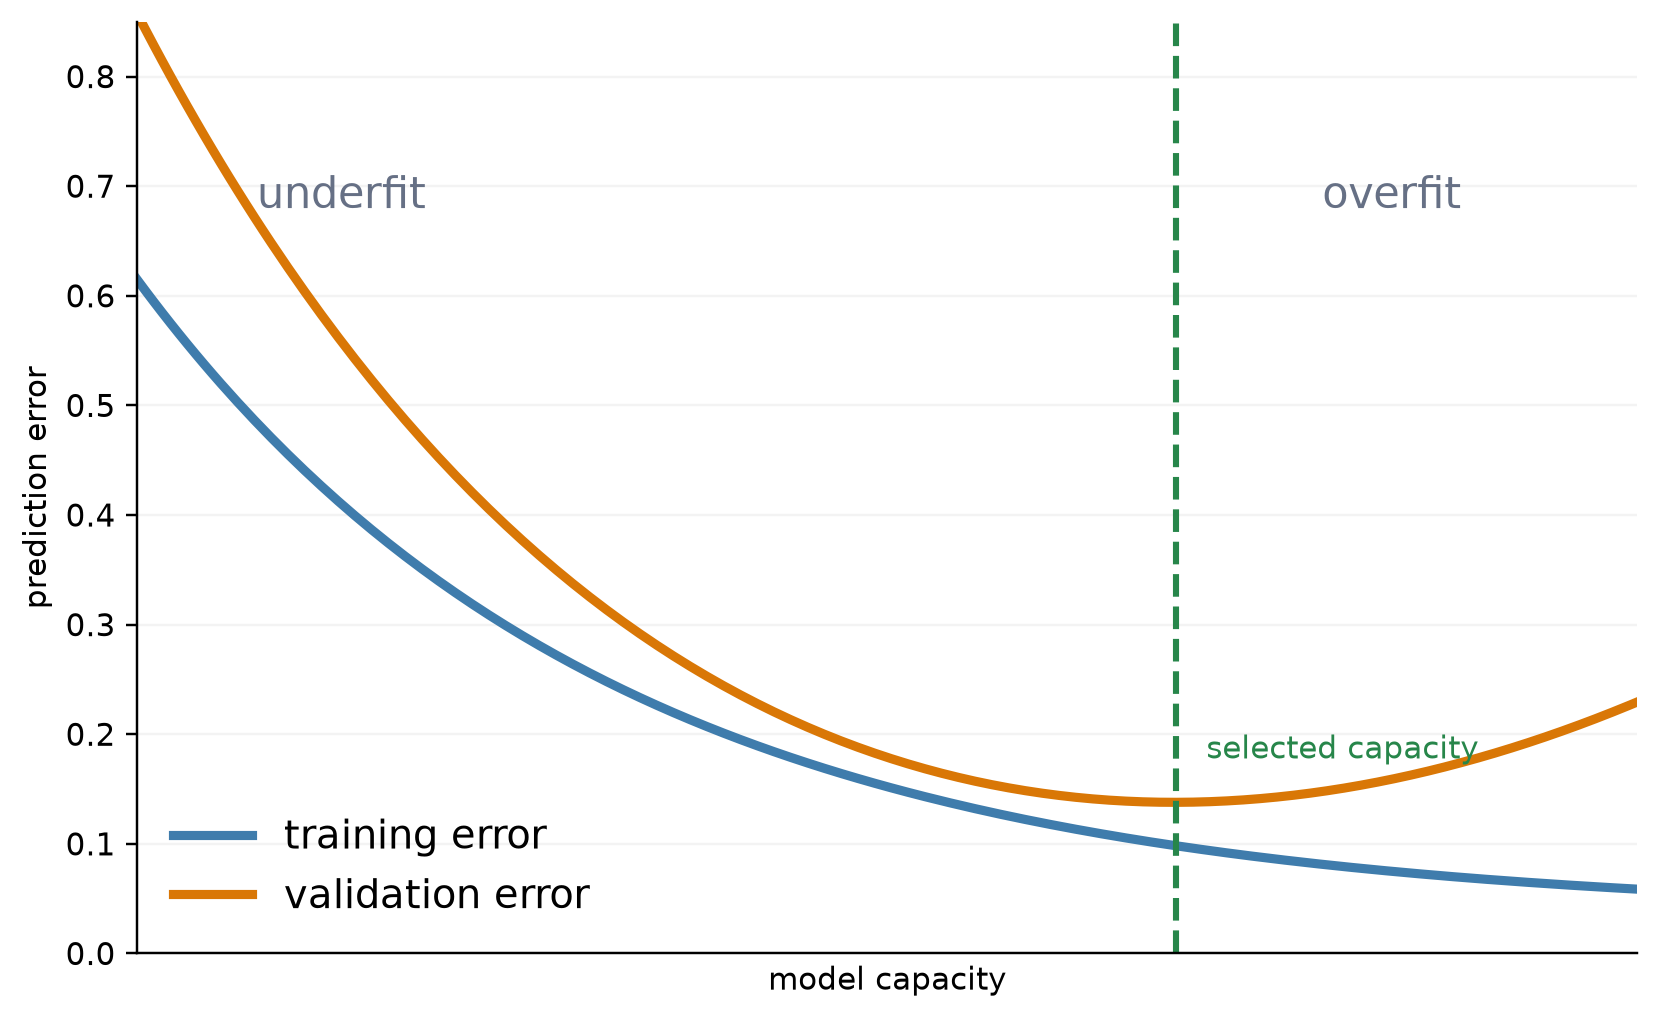
\includegraphics[width=0.9\linewidth,height=0.54\textheight,keepaspectratio]{learning-curves.png}

  \small Schematic. Capacity means how flexible the model is (for example, the polynomial degree or the number of weights).
  \takeaway{So: training error keeps falling with capacity, validation error falls and then rises; we want the bottom.}
\end{frame}


% ------------------------------------------------------------------ bias and variance
\section{Bias and Variance}
\sectiondivider{Bias and Variance}

\begin{frame}{Bias: The Average Fit Misses the Truth}
  At a fixed input $x$, let $f(x)=\mathbb E[Y\mid X=x]$ and
  $\bar f(x)=\mathbb E_D[\widehat f_D(x)]$, the average fit over random training sets $D$.
  \[
    \operatorname{Bias}[\widehat f(x)]=\bar f(x)-f(x).
  \]
  A rigid model can miss $f(x)$ in the same direction across datasets. More samples alone do not repair an inadequate model class.
\end{frame}

\begin{frame}{Variance: The Fit Changes with the Dataset}
  Refit the same learning procedure on a new sample $D$: its prediction at $x$ may move.
  \[
    \operatorname{Var}[\widehat f(x)]
    =\mathbb E_D\!\left[(\widehat f_D(x)-\bar f(x))^2\right].
  \]
  High variance means that the fitted prediction is sensitive to which training examples happened to be observed.
\end{frame}

\begin{frame}{The Four Cases as a Target}
  \centering
  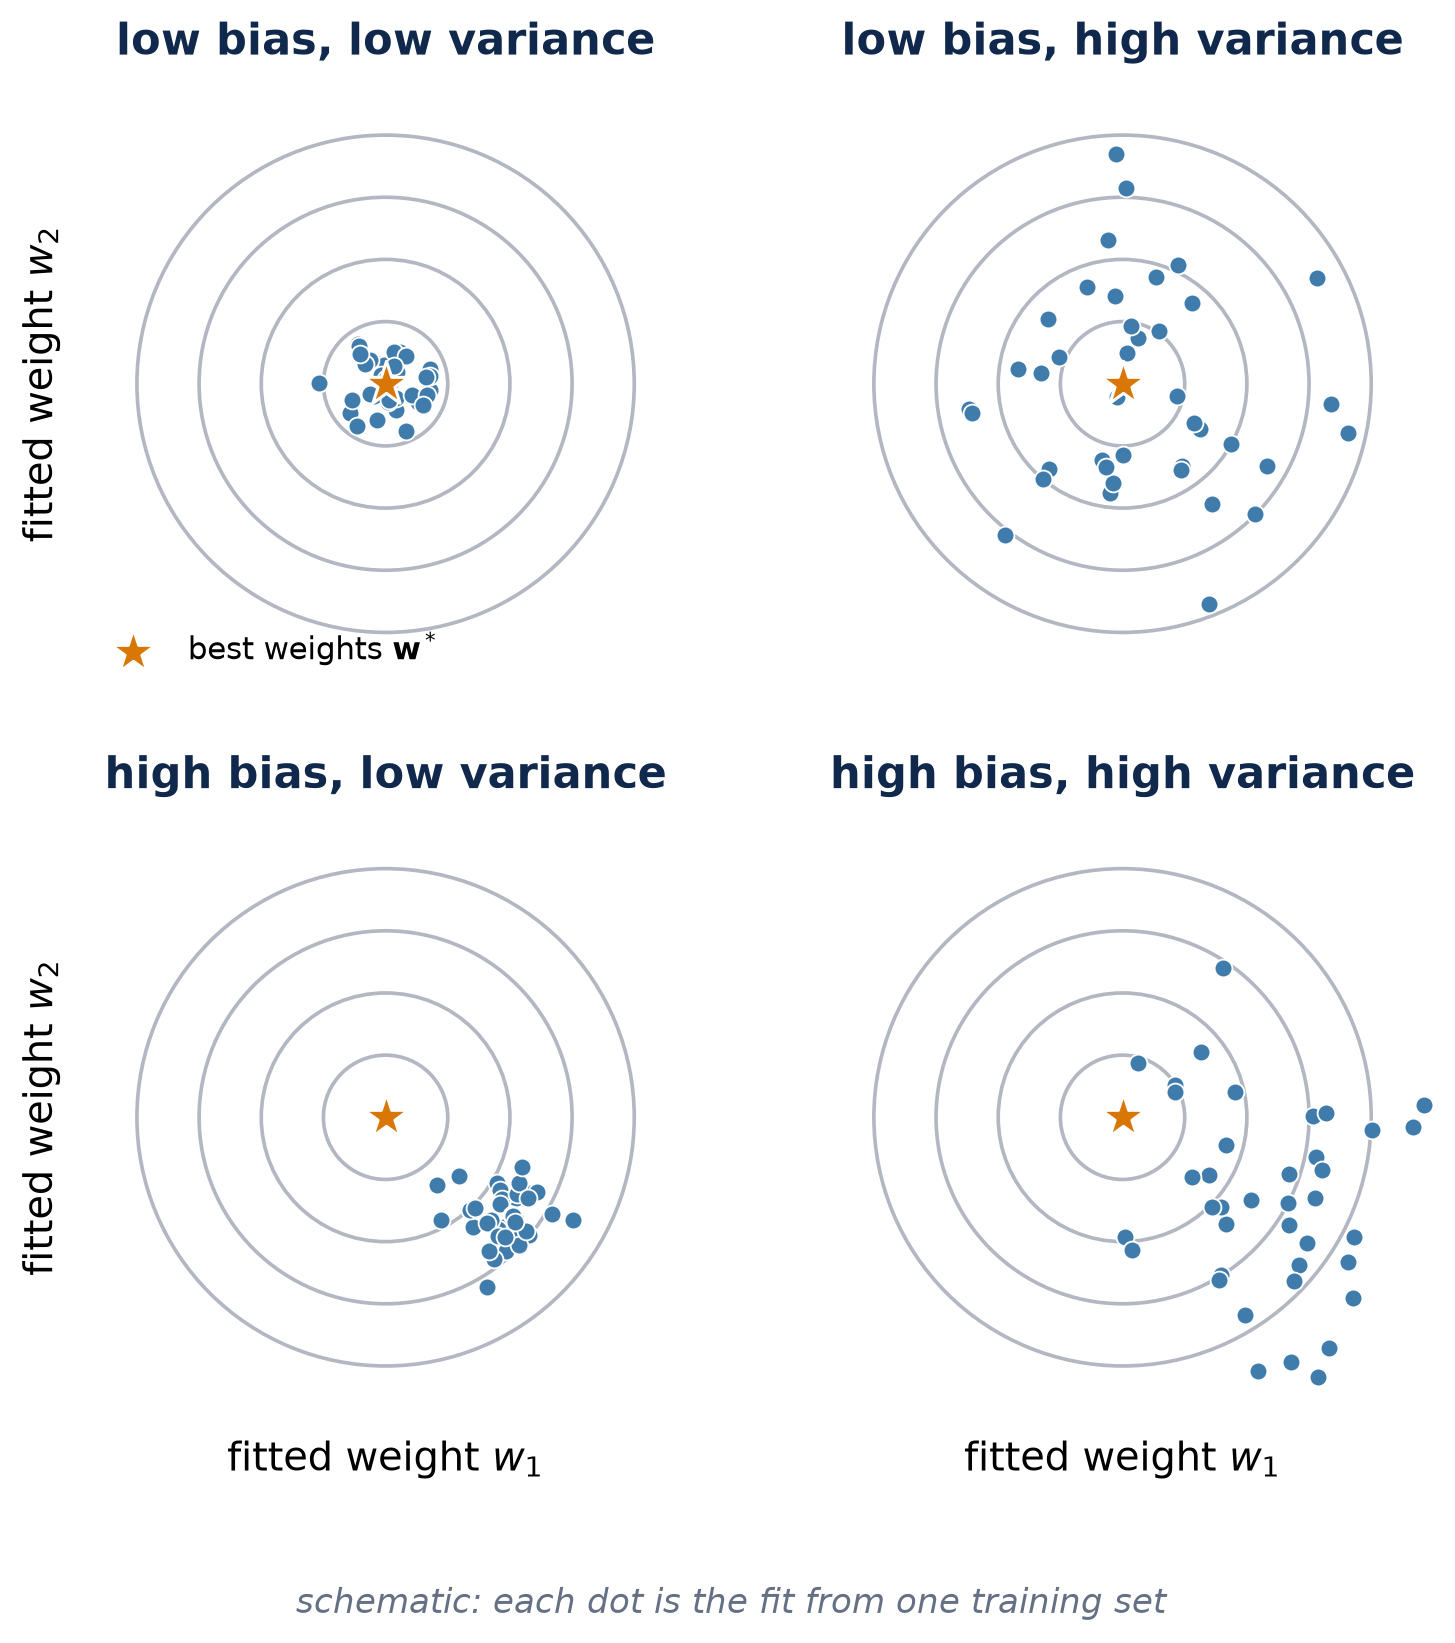
\includegraphics[height=0.66\textheight,keepaspectratio]{bias-variance-targets.png}
  \takeaway{So: low bias means the cloud is centered on the bullseye; low variance means the cloud is tight.}
\end{frame}

\begin{frame}{The Same Idea in Prediction Space}
  \centering
  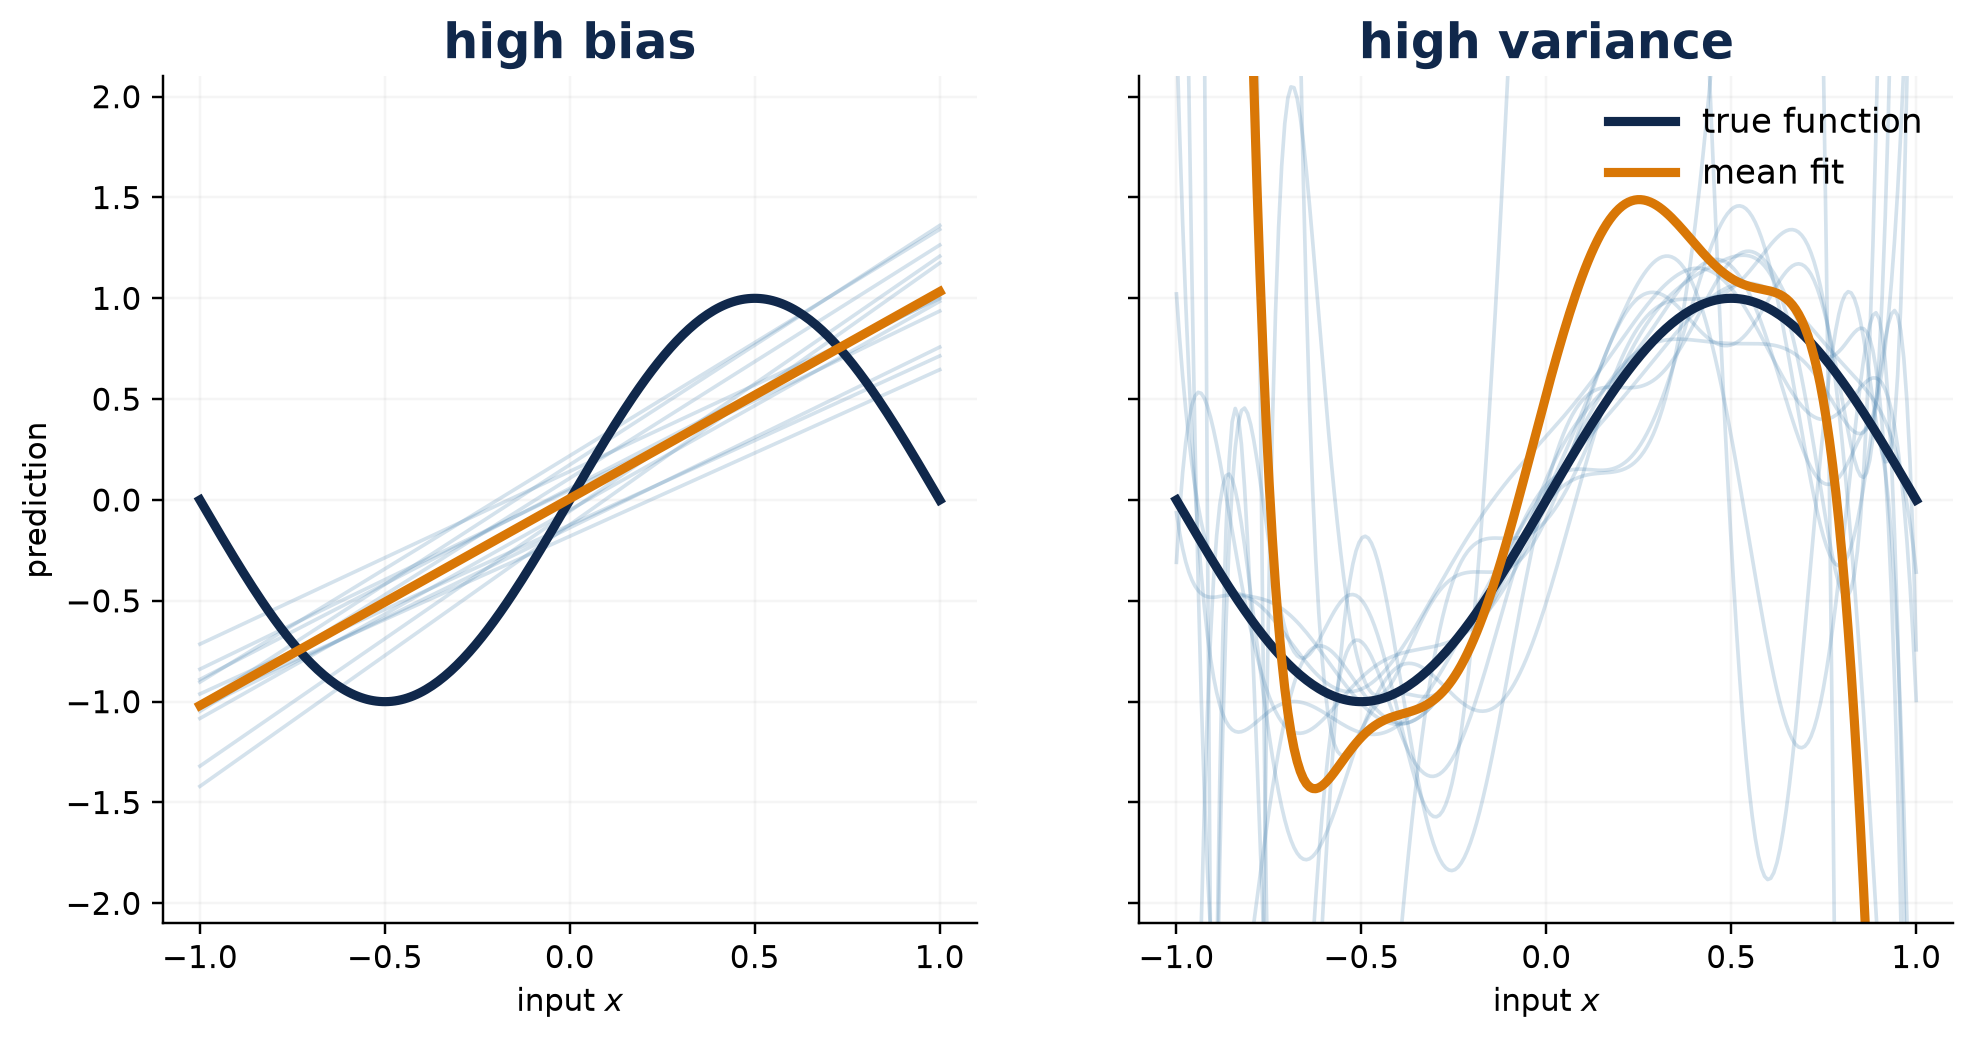
\includegraphics[width=0.98\linewidth,height=0.52\textheight,keepaspectratio]{bias-variance.png}

  \small Each thin curve is the fit from one of 12 training sets; the orange curve is their average.
  \takeaway{So: the line is stable but its average misses the curve (bias); the degree-9 fits scatter widely (variance).}
\end{frame}

\begin{frame}{Flexibility Trades One for the Other}
  \begin{center}
    \begin{tabular}{lcc}
      \toprule
      & \textbf{bias} & \textbf{variance}\\
      \midrule
      simple, rigid model & high & low\\
      flexible model & low & high\\
      \bottomrule
    \end{tabular}
  \end{center}
  \begin{itemize}
    \item Adding flexibility lets the average fit match the truth (less bias) but makes it follow each sample (more variance).
    \item More data lowers variance; it does not lower bias.
  \end{itemize}
  \takeaway{So: choosing model flexibility is choosing a balance between bias and variance.}
\end{frame}

\begin{frame}{Total Error Has Three Parts}
  Assume $Y=f(X)+\varepsilon$ with $\mathbb E[\varepsilon\mid X]=0$, and let the new observation be independent of the training set $D$.
  At a fixed $x$, write $\sigma^2(x)=\operatorname{Var}(Y\mid X=x)$. Then:
  \[
    \begin{aligned}
    \mathbb E_{D,Y\mid x}[(Y-\widehat f_D(x))^2]
      ={}&(\bar f(x)-f(x))^2\\
       &+\mathbb E_D[(\widehat f_D(x)-\bar f(x))^2]+\sigma^2(x)\\
      ={}&\operatorname{Bias}[\widehat f(x)]^2
       +\operatorname{Var}[\widehat f(x)]+\sigma^2(x).
    \end{aligned}
  \]
  The learning method can trade the first two terms; it cannot remove randomness in $Y$ given $X=x$.
\end{frame}

\begin{frame}{Diagnose Before You Fix}
  \begin{center}
    \small
    \begin{tabular}{llll}
      \toprule
      \textbf{training error} & \textbf{validation error} & \textbf{gap} & \textbf{diagnosis}\\
      \midrule
      high & high & small & high bias (underfit)\\
      low & high & large & high variance (overfit)\\
      low & low & small & good fit\\
      \bottomrule
    \end{tabular}
  \end{center}
  \begin{itemize}
    \item High training error: the model cannot even fit what it sees, so the cause is bias.
    \item Large train-validation gap: it fits the sample but not new data, so the cause is variance.
  \end{itemize}
  \takeaway{So: read the two errors first; the pattern tells you which remedy to try.}
\end{frame}

\begin{frame}{The Remedy Depends on the Diagnosis}
  \begin{columns}[T]
    \column{0.48\textwidth}
    \textbf{High bias}
    \begin{itemize}
      \item Use a more flexible model.
      \item Add informative features.
      \item Train longer or optimize better.
      \item Weaken regularization.
    \end{itemize}
    \column{0.48\textwidth}
    \textbf{High variance}
    \begin{itemize}
      \item Get more data.
      \item Add regularization.
      \item Stop training earlier.
      \item Average several models.
      \item Use dropout.
    \end{itemize}
  \end{columns}
  \takeaway{So: the rest of the lecture is the right-hand column; the wrong remedy makes things worse.}
\end{frame}


% ------------------------------------------------------------------ regularization
\section{Controlling Variance with Penalties}
\sectiondivider{Controlling Variance with Penalties}

\begin{frame}{The Regularized Objective}
  \[
    L_\lambda(\mathbf w,b)=L_{\mathrm{data}}(\mathbf w,b)+\lambda\Omega(\mathbf w),
    \qquad \lambda\ge0.
  \]
  \begin{center}
    \begin{tabular}{ll}
      \toprule
      L2 (ridge) & $\Omega(\mathbf w)=\|\mathbf w\|_2^2$\\
      L1 (lasso) & $\Omega(\mathbf w)=\|\mathbf w\|_1$\\
      \bottomrule
    \end{tabular}
  \end{center}
  Choose $\lambda$ on validation data. The intercept $b$ is excluded from the penalty, while the weights must earn their size through a better fit.
\end{frame}

\begin{frame}{Choosing the Strength $\lambda$}
  \begin{center}
    \small
    \begin{tabular}{lll}
      \toprule
      $\lambda$ & \textbf{what happens} & \textbf{failure}\\
      \midrule
      $0$ & no penalty, weights free & overfit\\
      moderate & weights shrunk, fit still follows the pattern & good fit\\
      very large & weights forced near $0$ & underfit\\
      \bottomrule
    \end{tabular}
  \end{center}
  Try several values of $\lambda$, train on the training set, and keep the one with the lowest
  \emph{validation} error. The test set is touched once, at the very end.
  \takeaway{So: $\lambda$ is itself a bias-variance dial, set with validation data.}
\end{frame}

\begin{frame}{The Compromise as a Picture}
  \centering
  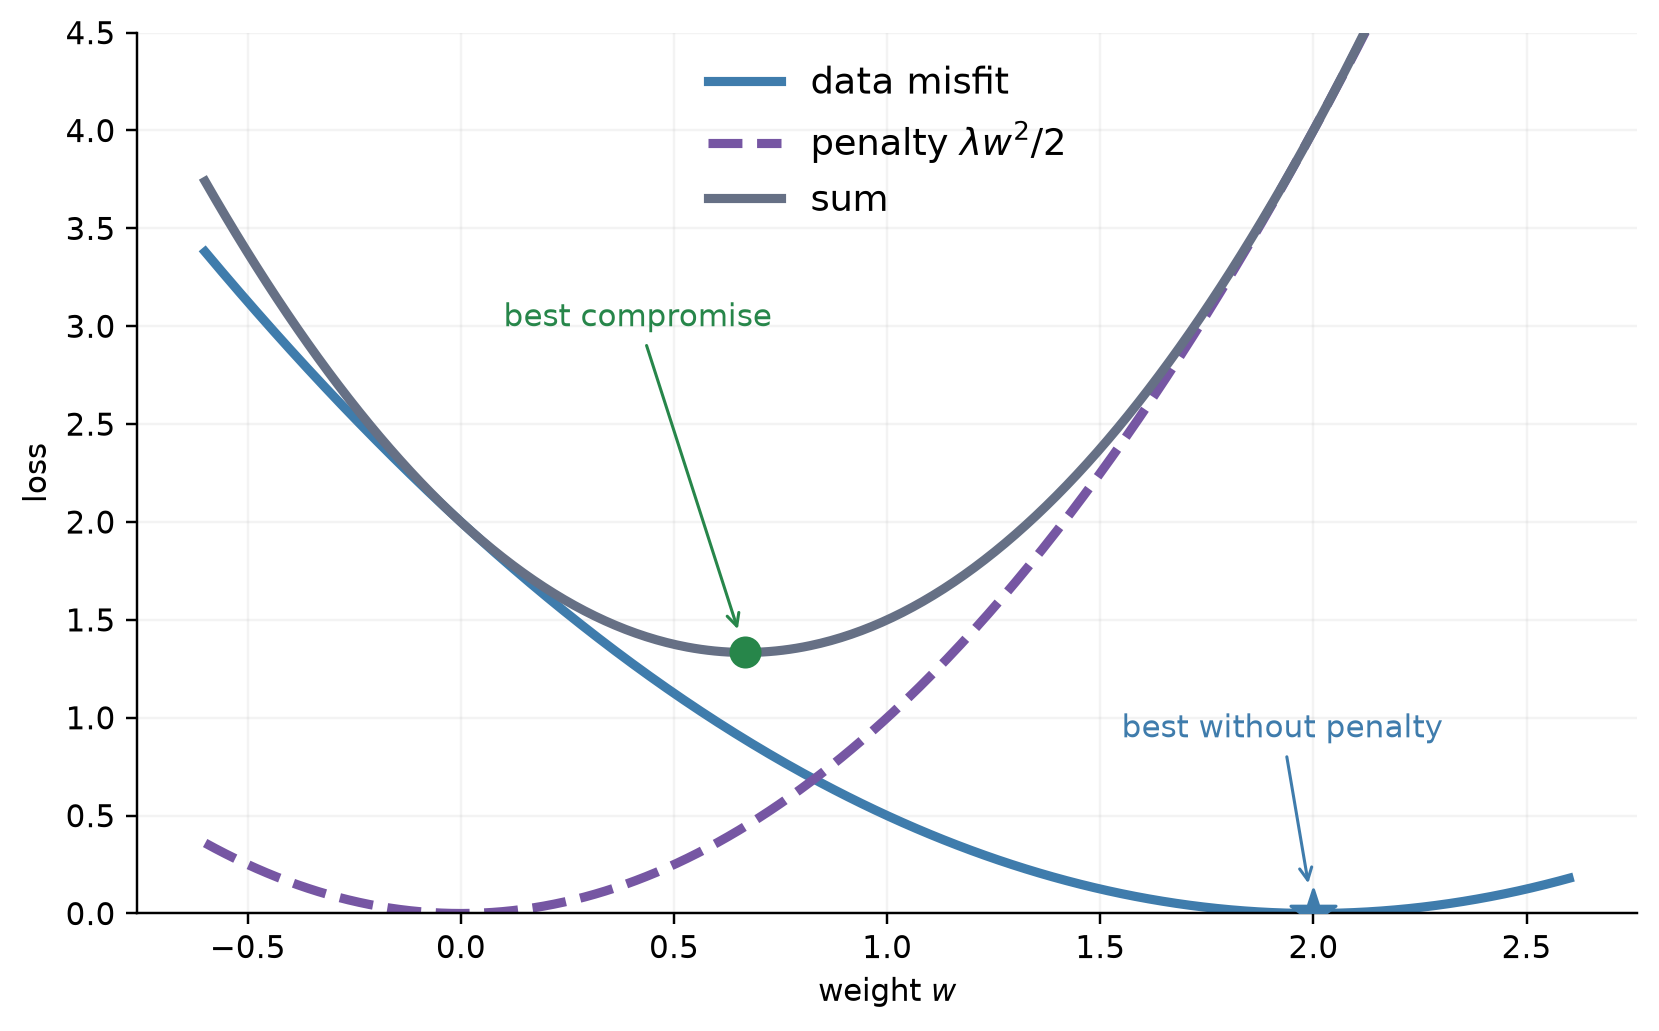
\includegraphics[width=0.8\linewidth,height=0.62\textheight,keepaspectratio]{l2-one-weight.png}
  \takeaway{So: adding the two parabolas gives a new bowl whose bottom lies between their bottoms.}
\end{frame}

\begin{frame}{L2: Penalize the Squared Weights}
  \[
    \Omega_{\mathrm{L2}}(\mathbf w)=w_1^2+w_2^2+\dots=\|\mathbf w\|_2^2 .
  \]
  Big weights are punished heavily, small ones barely. The result: \emph{all} weights shrink smoothly toward zero
  (in linear models this is called ridge regression).
  \takeaway{So: L2 shrinks weights smoothly; it does not generally create exact zeros.}
\end{frame}

\begin{frame}{L2 Picture: The Minimum Moves Toward Zero}
  \begin{columns}[c]
    \column{0.56\textwidth}
    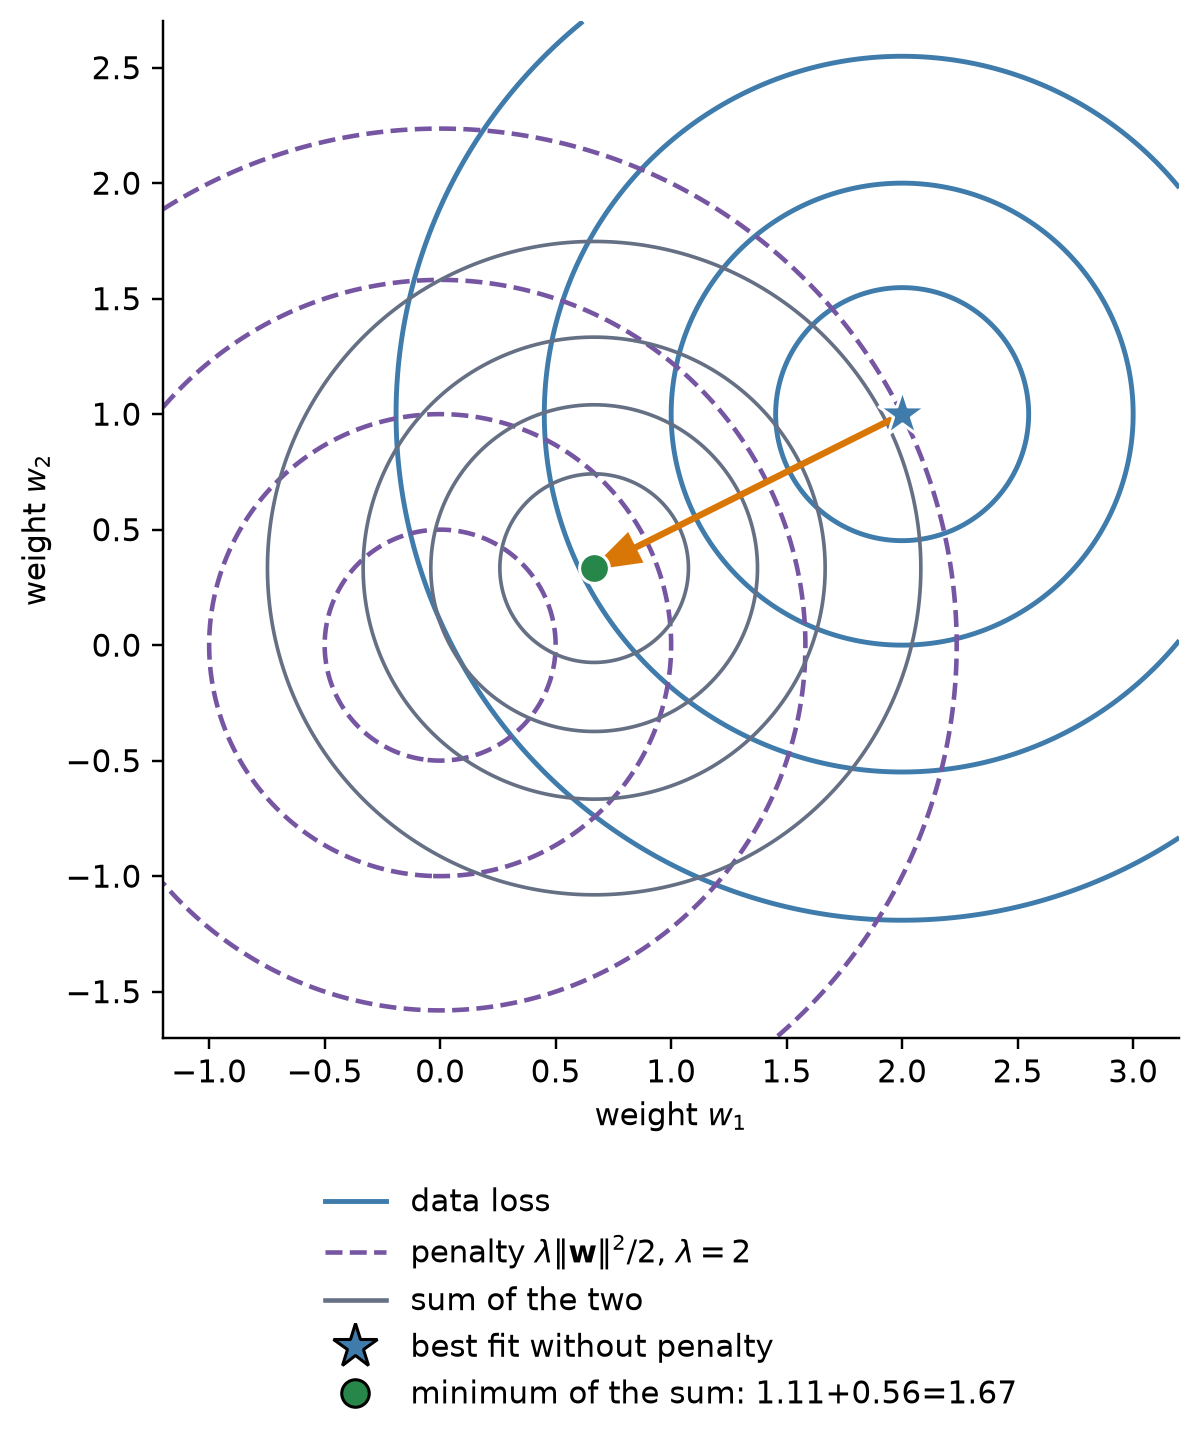
\includegraphics[width=\linewidth,height=0.66\textheight,keepaspectratio]{l2-contours.png}
    \column{0.42\textwidth}
    \small
    Gray contours show the sum, as heights above its minimum ($+0.25,+0.75,+1.5,+3.0$).
    \medskip

    At the green point: data misfit $1.11$ + penalty $0.56$ = sum $1.67$.
    \medskip

    The arrow shows the shift from the data-only best fit to the compromise.
  \end{columns}
  \takeaway{So: with two weights too, the best compromise lies between the data-only optimum and the origin.}
\end{frame}

\begin{frame}{L2 Worked Example}
  Two weights; the data alone would choose $(w_1,w_2)=(2,1)$. For the loss
  $\tfrac12\|\mathbf w-(2,1)\|^2+\tfrac{\lambda}{2}\|\mathbf w\|^2$ the minimum is $(2,1)/(1+\lambda)$.
  \begin{center}
    \begin{tabular}{rcc}
      \toprule
      $\lambda$ & $(w_1,w_2)$ & distance from origin\\
      \midrule
      0 & $(2.00,\ 1.00)$ & 2.24\\
      1 & $(1.00,\ 0.50)$ & 1.12\\
      2 & $(0.67,\ 0.33)$ & 0.75\\
      9 & $(0.20,\ 0.10)$ & 0.22\\
      \bottomrule
    \end{tabular}
  \end{center}
  \small This closed form holds for this simple quadratic example only.
  \takeaway{So: a larger $\lambda$ shrinks the weights further, all by the same factor.}
\end{frame}

\begin{frame}{Regularization Path: Weights versus $\lambda$}
  \centering
  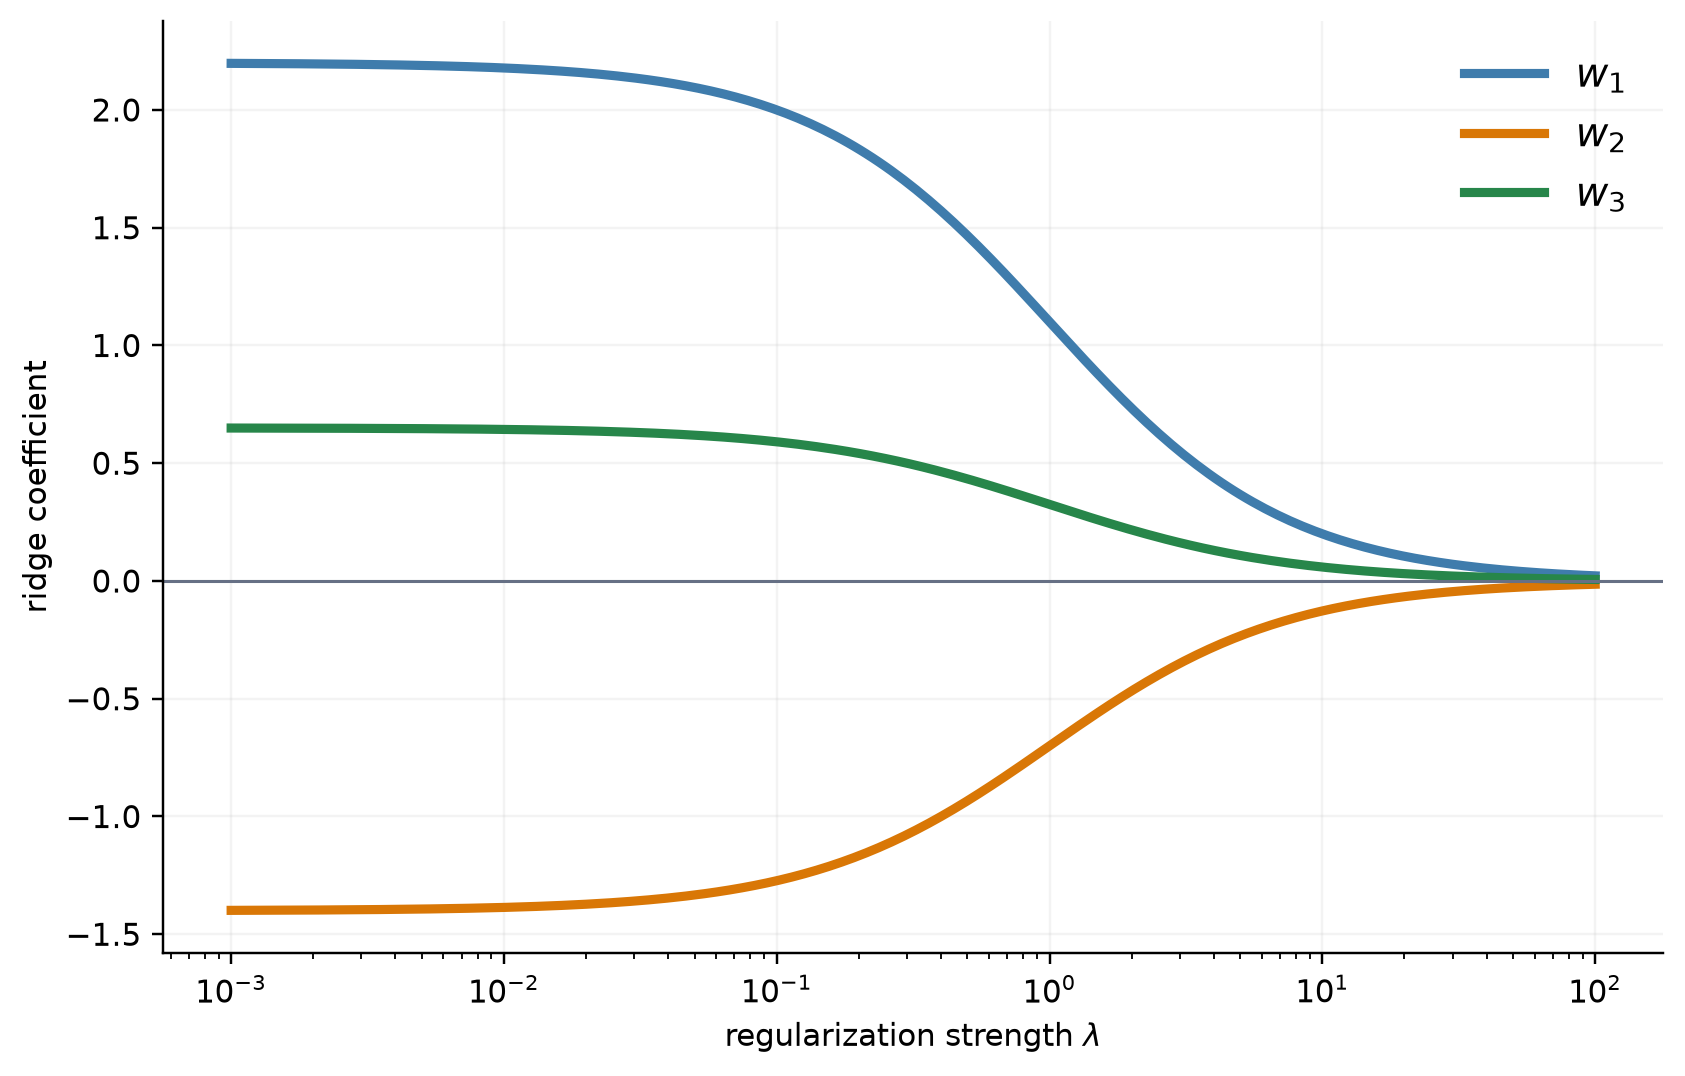
\includegraphics[width=0.85\linewidth,height=0.66\textheight,keepaspectratio]{regularization-path.png}
  \takeaway{So: as $\lambda$ grows, all coefficients shrink smoothly and together.}
\end{frame}

\begin{frame}{L1: Penalize the Absolute Weights}
  \[
    \Omega_{\mathrm{L1}}(\mathbf w)=|w_1|+|w_2|+\dots=\|\mathbf w\|_1 .
  \]
  L1 charges the same price per unit of weight whether it is large or small, so a small weight is not
  ``almost free'' as under L2. Weights that matter little are pushed all the way to \textbf{exactly zero}
  (in linear models this is called the lasso).
  \takeaway{So: L1 switches features off; the model keeps only the inputs that earn their place.}
\end{frame}

\begin{frame}{Another View: Weights Must Stay Inside a Shape}
  Instead of adding a penalty, we can say: the weights must stay inside a shape, and we take the best fit that is allowed.
  \centering
  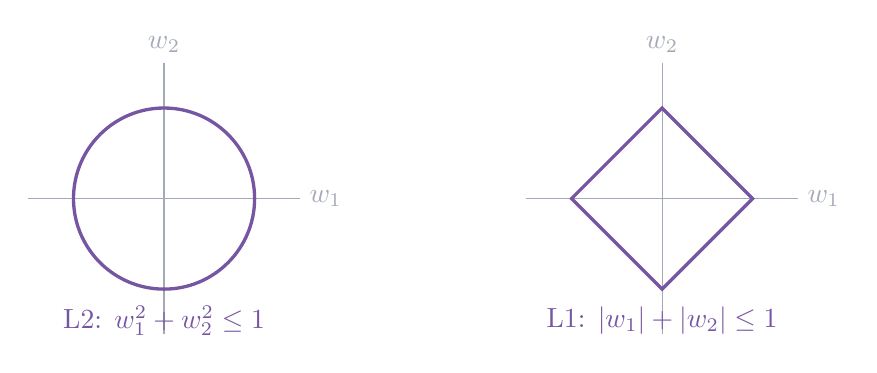
\begin{tikzpicture}[scale=1.15]
    \draw[coursegray!60] (-1.5,0)--(1.5,0) node[right]{$w_1$}; \draw[coursegray!60] (0,-1.5)--(0,1.5) node[above]{$w_2$};
    \draw[coursepurple,very thick] (0,0) circle (1);
    \node[coursepurple] at (0,-1.35) {L2: $w_1^2+w_2^2\le 1$};
    \begin{scope}[xshift=5.5cm]
      \draw[coursegray!60] (-1.5,0)--(1.5,0) node[right]{$w_1$}; \draw[coursegray!60] (0,-1.5)--(0,1.5) node[above]{$w_2$};
      \draw[coursepurple,very thick] (1,0)--(0,1)--(-1,0)--(0,-1)--cycle;
      \node[coursepurple] at (0,-1.35) {L1: $|w_1|+|w_2|\le 1$};
    \end{scope}
  \end{tikzpicture}

  \raggedright\small A smaller shape means a stronger penalty (a larger $\lambda$): the two views give the same family of solutions.
  \takeaway{So: L2 allows a disk of weights, L1 a diamond; the diamond has corners on the axes.}
\end{frame}

\begin{frame}{Best Allowed Weights}
  \centering
  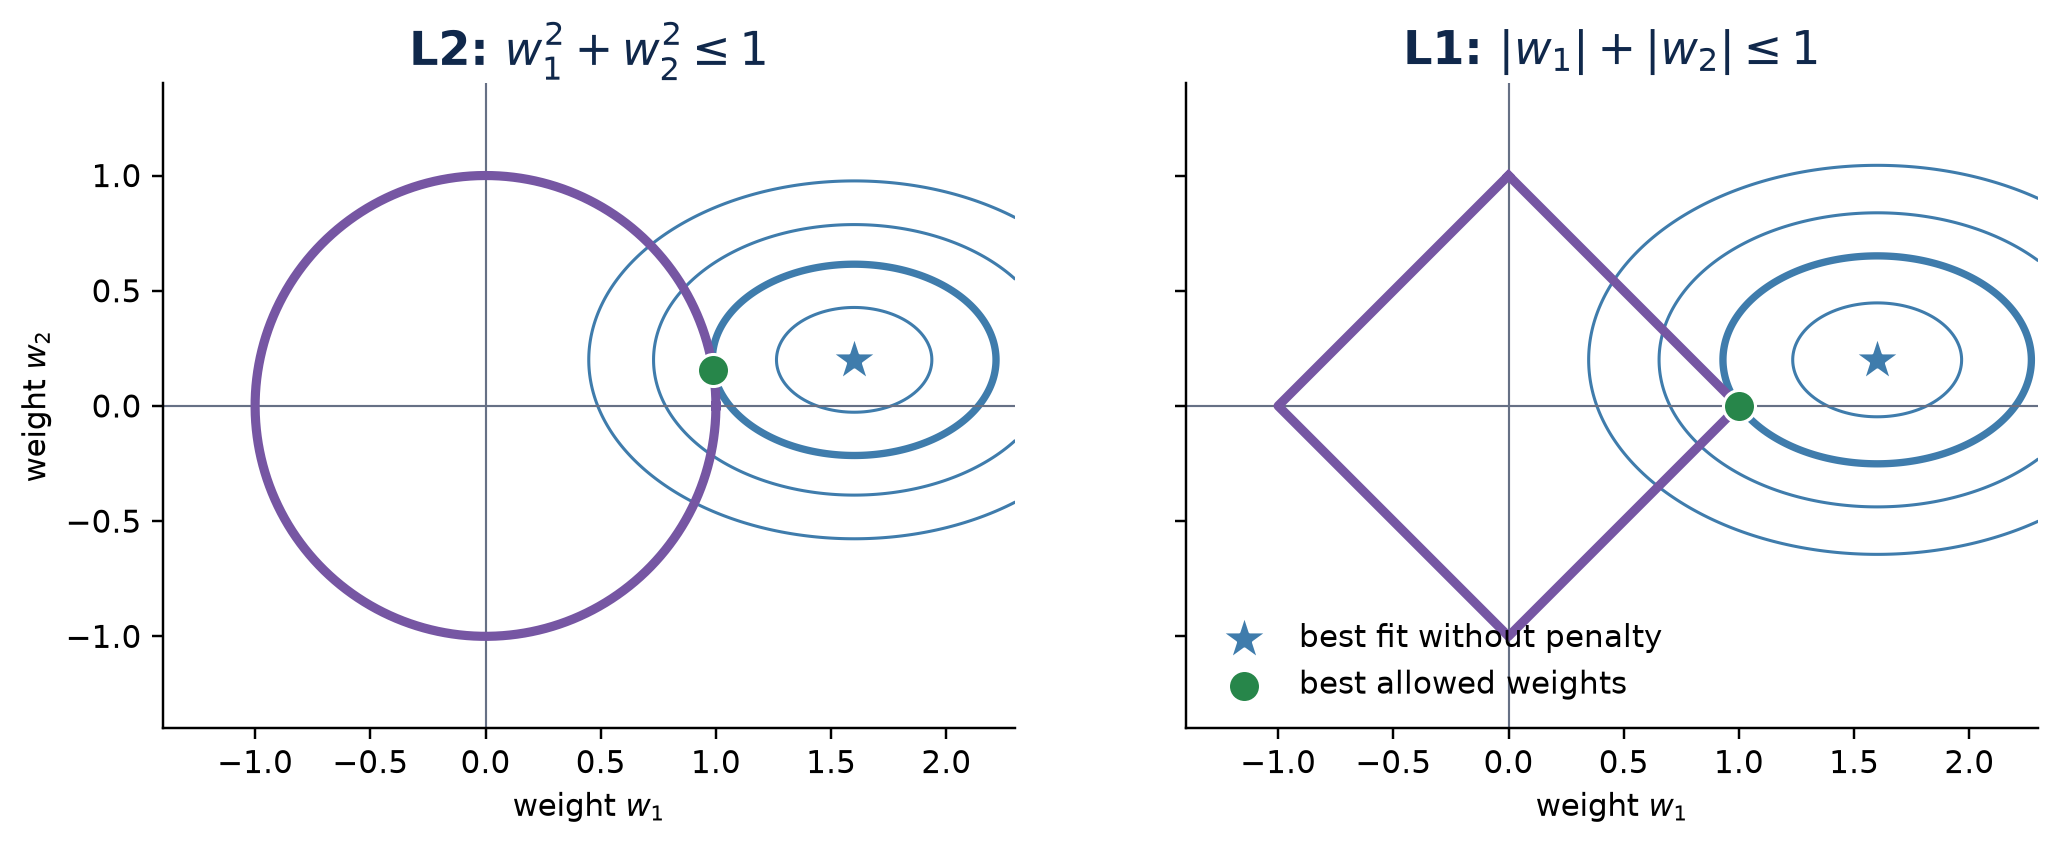
\includegraphics[width=0.98\linewidth,height=0.55\textheight,keepaspectratio]{l1-l2-geometry.png}

  \small Blue ellipses: loss contours around the best fit without penalty (star), which lies outside the shape.
  The thick contour is the lowest loss that still touches the shape.
  \takeaway{So: the best allowed point is where the lowest loss contour first touches the shape.}
\end{frame}

\begin{frame}{Why the Diamond Gives Exact Zeros}
  \begin{itemize}
    \item The circle has no corners: the contour touches it at a generic point, so both weights stay nonzero (here $w_2\approx0.16$).
    \item The diamond's corners lie \emph{on the axes}. A contour from a far-away optimum tends to touch a corner first.
    \item At a corner one weight is exactly $0$: here $(w_1,w_2)=(1,0)$.
  \end{itemize}
  \small In this example the best fit without penalty is $(1.6,\,0.2)$; the numbers are computed, not drawn by hand.
  \takeaway{So: L1 switches a weight off exactly; L2 only makes it small.}
\end{frame}

\begin{frame}{L1 or L2?}
  \begin{center}
    \small
    \begin{tabular}{lp{3.3cm}p{3.3cm}}
      \toprule
      & \textbf{L2} & \textbf{L1}\\
      \midrule
      Penalty & sum of squares & sum of absolute values\\
      Weights become & small & small, many exactly $0$\\
      Use when & many weak useful inputs & few inputs matter; want selection\\
      \bottomrule
    \end{tabular}
  \end{center}
  \takeaway{So: L2 is the default smoother; choose L1 when you want a sparse, easier-to-read model.}
\end{frame}

\begin{frame}{Penalize the Weights, Not the Intercept}
  \[
    \hat y=\mathbf w\cdot\mathbf x+b .
  \]
  The penalty is applied to $\mathbf w$ only.
  \begin{itemize}
    \item The intercept $b$ sets the overall level of the output; it does not make the fit wiggly.
    \item Shrinking $b$ toward zero would push every prediction toward $0$, which is bias with no variance benefit.
  \end{itemize}
  \takeaway{So: shrink the weights that control the shape of the fit; leave the intercept free.}
\end{frame}


% ------------------------------------------------------------------ early stopping
\section{Controlling Variance by Other Means}
\sectiondivider{Controlling Variance by Other Means}

\begin{frame}{Early Stopping: When Training Itself Overfits}
  Training is iterative. Early on, the model learns the broad pattern; later, it starts fitting the noise.
  \begin{itemize}
    \item Training error keeps falling with every epoch.
    \item Validation error falls, reaches a minimum, then rises.
  \end{itemize}
  \takeaway{So: the longer we train, the more flexible the fitted model effectively becomes.}
\end{frame}

\begin{frame}{Early Stopping: Keep the Best Iterate}
  \centering
  \begin{tikzpicture}
    \begin{axis}[width=0.85\linewidth,height=0.58\textheight,xmin=0,xmax=10,ymin=0,ymax=1,
      xlabel={training epoch},ylabel={error},grid=both,legend style={draw=none,at={(0.98,0.98)},anchor=north east}]
      \addplot[courseblue,very thick,domain=0:10,samples=100] {0.75*exp(-0.35*x)+0.05};
      \addlegendentry{training}
      \addplot[courseorange,very thick,domain=0:10,samples=100] {0.55*exp(-0.5*x)+0.12+0.012*(x-4.7)^2};
      \addlegendentry{validation}
      \draw[coursegreen,very thick,dashed] (axis cs:5.45,0)--(axis cs:5.45,0.75);
      \node[coursegreen,font=\bfseries] at (axis cs:6.55,0.72) {restore best};
    \end{axis}
  \end{tikzpicture}

  \small Schematic curves. Watch validation error each epoch; if it has not improved for a set number of epochs, stop and restore the best weights.
  \takeaway{So: stopping at the validation minimum acts like regularization and costs nothing extra.}
\end{frame}

% ------------------------------------------------------------------ ensembles
\begin{frame}{Ensembles: Ask Several Models and Average}
  One model's variance is its sensitivity to the sample. Several models trained differently make
  different mistakes, and the mistakes partly cancel.
  \begin{center}
    \small
    \begin{tabular}{lcccccc}
      \toprule
      & m1 & m2 & m3 & m4 & m5 & \textbf{average}\\
      \midrule
      prediction (true value $10$) & 7 & 12 & 9 & 13 & 8 & \textbf{9.8}\\
      error & $-3$ & $+2$ & $-1$ & $+3$ & $-2$ & \textbf{$-0.2$}\\
      \bottomrule
    \end{tabular}
  \end{center}
  \takeaway{So: each model is off by 1 to 3, the average is off by 0.2, because the errors point in different directions.}
\end{frame}

\begin{frame}{When Averaging Helps}
  \begin{itemize}
    \item It helps when the models make \emph{different} mistakes; five copies of the same model gain nothing.
    \item It reduces variance. It does not remove bias that all models share.
    \item The models must each be reasonably good; averaging bad models stays bad.
  \end{itemize}
  The exact formula for the variance of an average is in the appendix.
  \takeaway{So: averaging attacks variance, and it works best with diverse, individually decent models.}
\end{frame}

\begin{frame}{Bagging: Diverse Models from One Dataset}
  We have only one dataset, so how do we get different models? Resample it.
  \textbf{Bootstrap sample:} draw $n$ points \emph{with replacement} from the $n$ we have.
  \begin{center}
    \small
    \begin{tabular}{ll}
      \toprule
      original data & a, b, c, d, e\\
      bootstrap 1 & b, b, d, e, e\\
      bootstrap 2 & a, c, c, d, a\\
      bootstrap 3 & e, a, b, b, c\\
      \bottomrule
    \end{tabular}
  \end{center}
  Each sample repeats some points and misses others, so each model sees slightly different data.
  \takeaway{So: resampling with replacement gives us many plausible datasets from the one we hold.}
\end{frame}

\begin{frame}{Bagging: Train on Each, Then Average}
  \centering
  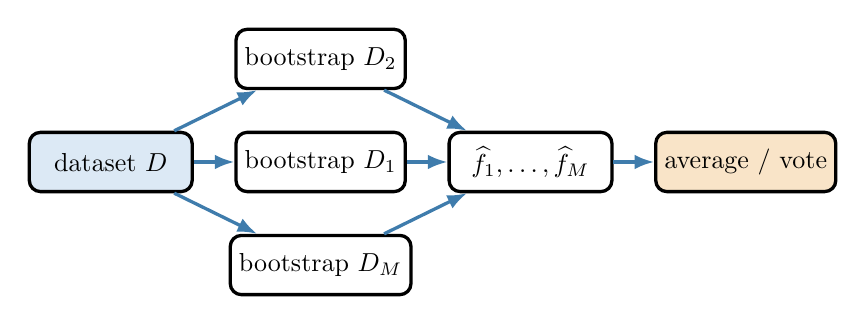
\begin{tikzpicture}[scale=0.94,transform shape,node distance=0.55cm,
    box/.style={draw,rounded corners,minimum width=2.2cm,minimum height=0.8cm,very thick,align=center},
    flow/.style={-{Latex[length=2.5mm]},very thick,courseblue}]
    \node[box,fill=courselightblue] (data) {dataset $D$};
    \node[box,right=of data] (b1) {bootstrap $D_1$};
    \node[box,above=of b1] (b2) {bootstrap $D_2$};
    \node[box,below=of b1] (bm) {bootstrap $D_M$};
    \node[box,right=of b1] (models) {$\widehat f_1,\ldots,\widehat f_M$};
    \node[box,fill=courselightorange,right=of models] (avg) {average / vote};
    \draw[flow] (data)--(b1); \draw[flow] (data)--(b2); \draw[flow] (data)--(bm);
    \draw[flow] (b1)--(models); \draw[flow] (b2)--(models); \draw[flow] (bm)--(models);
    \draw[flow] (models)--(avg);
  \end{tikzpicture}

  Regression: average the predictions. Classification: take a majority vote.
  \takeaway{So: bagging turns one unstable model into a steadier one at the price of training $M$ models.}
\end{frame}

% ------------------------------------------------------------------ dropout
\begin{frame}{Dropout: Do Not Let Units Rely on Each Other}
  In a neural network, a hidden unit can learn to fix the mistakes of its neighbors.
  Such units only work together; this fragile teamwork is a form of overfitting.
  \begin{itemize}
    \item \textbf{Idea:} during training, switch off a random subset of units at every step.
    \item Every unit must then be useful on its own, because its partners may be missing.
  \end{itemize}
  \takeaway{So: dropout forces the network to spread knowledge instead of relying on fragile combinations.}
\end{frame}

\begin{frame}{Dropout: A Different Smaller Network Each Step}
  \centering
  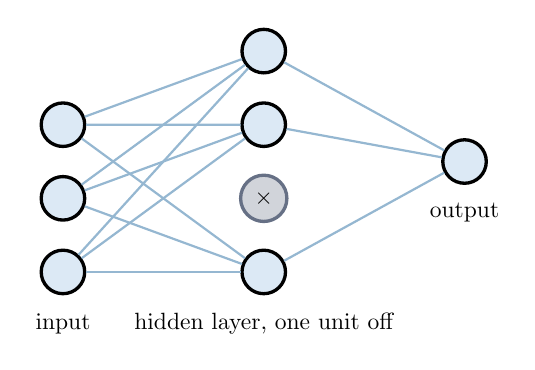
\begin{tikzpicture}[scale=0.85,transform shape,unit/.style={circle,draw,minimum size=0.65cm,very thick},
    kept/.style={unit,fill=courselightblue},dropped/.style={unit,fill=coursegray!30,draw=coursegray},
    edge/.style={courseblue!55,thick}]
    \foreach \y in {0,1,2}{\node[kept] (i\y) at (0,1.1*\y) {};}
    \node[kept] (h0) at (3,0) {}; \node[dropped] (h1) at (3,1.1) {$\times$};
    \node[kept] (h2) at (3,2.2) {}; \node[kept] (h3) at (3,3.3) {};
    \foreach \i in {0,1,2}{\foreach \h in {0,2,3}{\draw[edge] (i\i)--(h\h);}}
    \node[kept] (o) at (6,1.65) {};
    \foreach \h in {0,2,3}{\draw[edge] (h\h)--(o);}
    \node[below=0.15cm of i0] {input}; \node[below=0.15cm of h0] {hidden layer, one unit off};
    \node[below=0.15cm of o] {output};
  \end{tikzpicture}

  \[
    m_j\sim\operatorname{Bernoulli}(1-p),\qquad
    \widetilde h_j=\frac{m_jh_j}{1-p},\qquad
    \mathbb E_m[\widetilde h_j]=h_j.
  \]
  \small A fresh mask is sampled at each training step. The scaling preserves each activation's mean; at test time all units are used.
\end{frame}

% ------------------------------------------------------------------ summary
\begin{frame}{Match the Remedy to the Failure}
  \begin{center}
    \small
    \begin{tabular}{lp{5.4cm}}
      \toprule
      \textbf{Failure} & \textbf{Controls}\\
      \midrule
      high bias & richer model or features, longer or better training, weaker regularization\\
      high variance & more data, L2 or L1, early stopping, bagging and ensembles, dropout\\
      \bottomrule
    \end{tabular}
  \end{center}
  Choose every strength (\(\lambda\), stopping epoch, dropout rate) on validation data;
  use the test set once for the final estimate.
  \takeaway{So: diagnose from the train and validation errors first, then apply the matching control.}
\end{frame}


% ------------------------------------------------------------------ appendix
\appendix
\sectiondivider{Appendix: optional depth}

\begin{frame}{Appendix: The Cross Terms Vanish by Centering}
  Add and subtract $f(x)$ and $\bar f(x)=\mathbb E_D[\widehat f_D(x)]$:
  \[
    Y-\widehat f_D
    =\underbrace{Y-f}_{\varepsilon}
     +\underbrace{f-\bar f}_{-\mathrm{Bias}}
     +\underbrace{\bar f-\widehat f_D}_{\text{centered estimator}}.
  \]
  Squaring and taking expectations removes cross terms because
  \[
    \mathbb E[\varepsilon\mid x]=0,
    \qquad
    \mathbb E_D[\bar f-\widehat f_D]=0.
  \]
  The decomposition is exact under the stated squared-error assumptions.
\end{frame}

\begin{frame}{Appendix: L2 Is MAP under a Gaussian Prior}
  Assume independent weights and Gaussian observation noise:
  \[
    w_j\sim\mathcal N(0,\tau^2),
    \qquad
    y_i\mid\mathbf x_i,\mathbf w\sim
      \mathcal N(f_{\mathbf w}(\mathbf x_i),\sigma^2).
  \]
  Then
  \[
    -\log p(\mathbf w\mid D)
    =\frac1{2\sigma^2}\sum_i(y_i-f_{\mathbf w}(\mathbf x_i))^2
      +\frac1{2\tau^2}\|\mathbf w\|_2^2+\text{constant}.
  \]
  The zero mean expresses a prior preference for small weights, not knowledge that the true weights are zero.
\end{frame}

\begin{frame}{Appendix: Prior Scale and Strength of Belief}
  \centering
  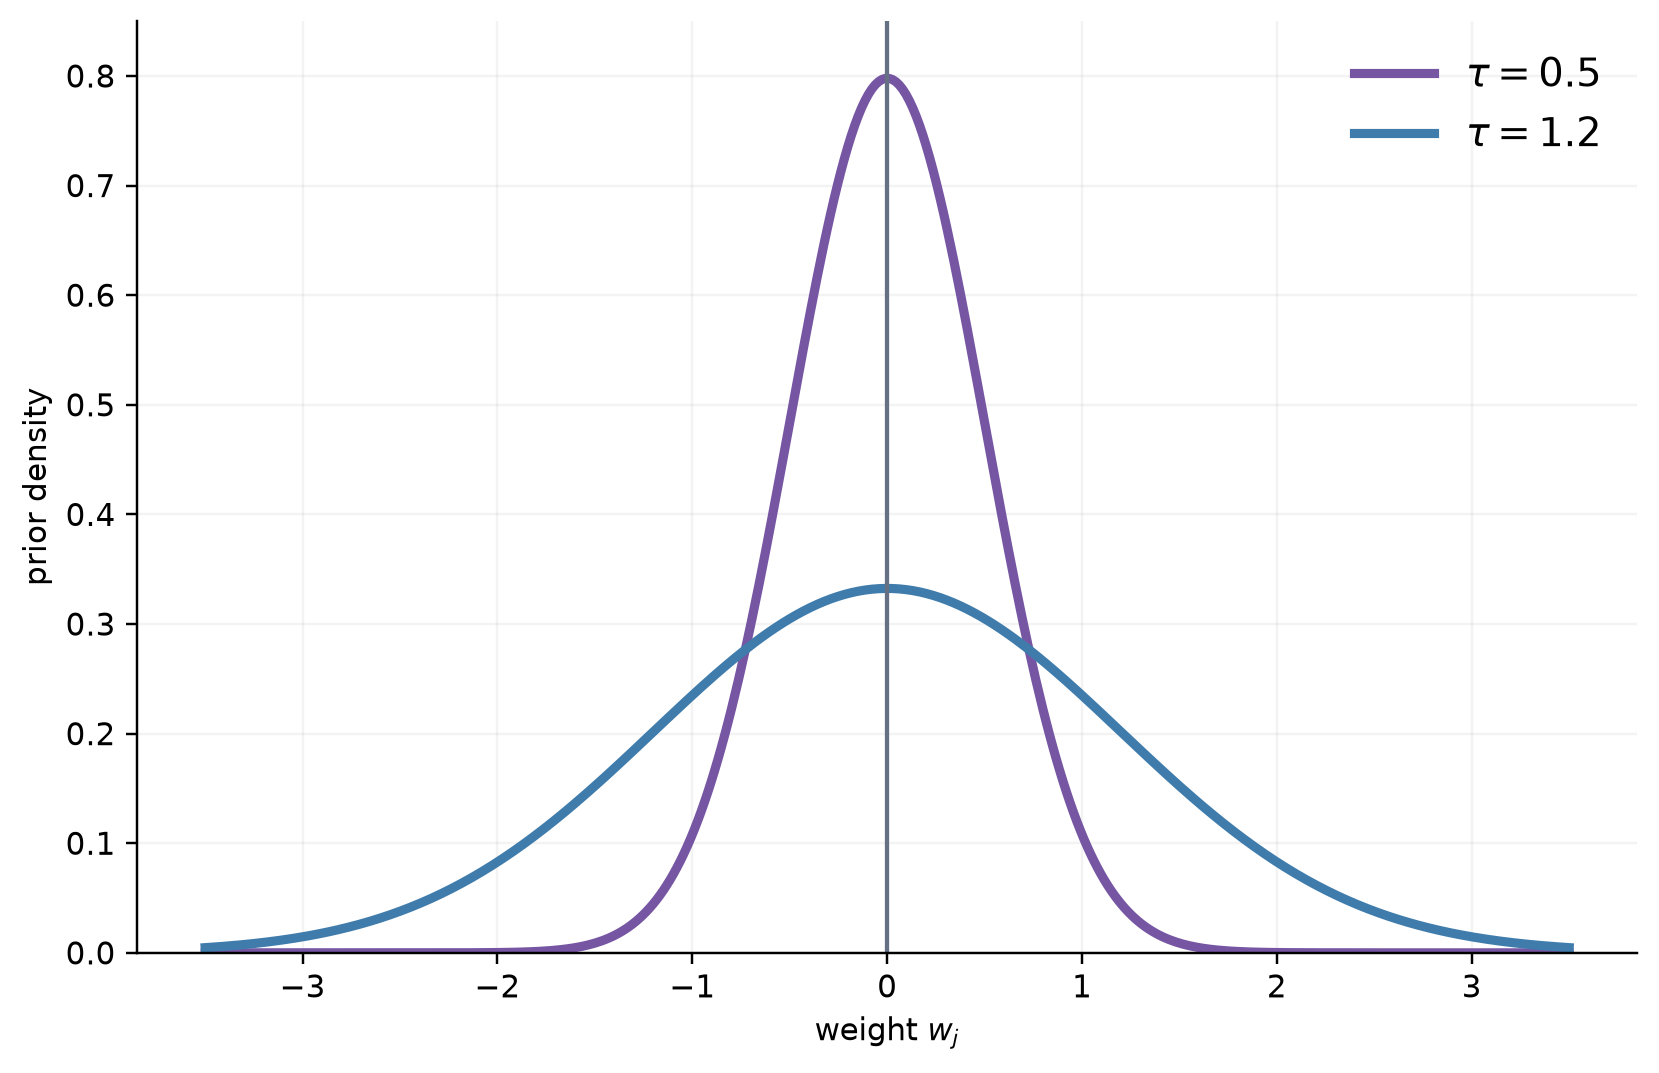
\includegraphics[width=0.9\linewidth,height=0.7\textheight,keepaspectratio]{weight-priors.png}

  \small A narrow prior ($\tau$ small) means a strong preference for small weights, that is, a large $\lambda$.
\end{frame}

\begin{frame}{Appendix: L1 Corresponds to a Laplace Prior}
  \[
    p(w_j)=\frac1{2b}\exp\!\left(-\frac{|w_j|}{b}\right)
    \quad\Longrightarrow\quad
    -\log p(\mathbf w)=\frac1b\|\mathbf w\|_1+\text{constant}.
  \]
  The L1 ball has corners on coordinate axes. A loss contour can first touch at a corner,
  so exact zeros are common in convex linear models.
  Neural-network parameter symmetries make sparsity effects less direct.
\end{frame}

\begin{frame}{Appendix: Variance of an Average of Predictors}
  Let $M$ predictors have equal variance $v$ and pairwise error correlation $\rho$.
  Their average has variance
  \[
    \operatorname{Var}\!\left(\frac1M\sum_{m=1}^M\widehat f_m\right)
    =v\left(\rho+\frac{1-\rho}{M}\right).
  \]
  With $\rho=0$ the variance falls like $1/M$; with $\rho=1$ averaging gains nothing.
  It does not remove shared bias.
\end{frame}

\begin{frame}{Appendix: Inverted Dropout Preserves the Mean}
  Let $\mathbf h$ be the vector of activations of a layer. For drop probability $p$, give each unit a random
  keep-indicator $m_j$ equal to $1$ with probability $1-p$ and $0$ otherwise, and use
  \[
    \widetilde h_j=\frac{m_j\,h_j}{1-p}.
  \]
  Averaged over many random draws of the indicators, $m_j$ averages to $1-p$, so
  \[
    \text{average of }\widetilde h_j=\frac{(1-p)\,h_j}{1-p}=h_j .
  \]
  This is the numeric example of the main slides in symbols. Dropout injects multiplicative noise; it does not guarantee independent features.
\end{frame}

\begin{frame}{Appendix: Monte Carlo Dropout}
  Standard inference uses the full network. A separate use of dropout keeps it \emph{on} at test time:
  \begin{enumerate}
    \item Run the same input through the network $T$ times, each with fresh random masks.
    \item Take the mean of the $T$ outputs as the prediction.
    \item Read their spread as a rough measure of uncertainty.
  \end{enumerate}
  This is an uncertainty heuristic, not the default inference rule, and it costs $T$ forward passes.
\end{frame}

\end{document}
